% -----------------------------*- LaTeX -*------------------------------
\documentclass[12pt]{report}
\input{header}
\usepackage{graphicx}
\graphicspath{ {Figures/} }
\usepackage{scribe_e1244}
\usepackage{times}
%\newtheorem{defn}[thm]{Definition}
%\newtheorem{lem}{Lemma}[thm]
%\newenvironment{definition}[1][Definition]{\begin{trivlist}
%\item[\hskip \labelsep {\bfseries #1}]}{\end{trivlist}}

\begin{document}

\lecturer{Aditya Gopalan}		
\scribe{Rinson Varghese \& Manju M Raj}	% required, put your name here
\lecturenumber{15}			% required, must be a number
\lecturedate{February 23}		% required, omit year
\maketitle

% title of the lecture
\begin{center}
{\Large \bf Sequential Detection   }
\end{center}
	
	
% ----------------------------------------------------------------------
% ----------------------------------------------------------------------

\section{Motivation}
So far we fixed sample size (${\underline{Y}} \in \mathbbm{R}^n$) and designed for performance ($r(.), P_F, P_M$). Alternatively we can also fix desired performance level and design for; without necessarily using a fixed sample size. In many cases we can do it with lesser number of samples. 


\section{Basic Model}

\begin{align*}
H_0 &: Y_k\stackrel{iid}\sim P_0,~k=1,2,\dots\\
versus\\
H_1 &: Y_k\stackrel{iid}\sim {P}_1,~k=1,2,\dots
\end{align*}
where $Y_k \in \mathbbm{R}$.
In general we have infinitely many samples available.
\section{Protocol of iteration}
At each time n = 0,1,2,\dots\ (time as a counter)\newline
\begin{itemize}
	\item Detector decides whether to stop taking samples or to continue, based on ($Y_1,Y_2,\dots\\ Y_n$)
	\item If STOP : ( i.e.\ $\phi_n(Y_1,Y_2,\cdots,Y_N)=1$), output decision ($\delta_N(Y_1,Y_2,\cdots,Y_N)$) based on samples ($Y_1,Y_2,\dots, Y_n$)
	\item Break
\end{itemize}
\begin{defn}
	A sequential decision rule is a pair of sequences of fuctions $(\underline{\phi},\;\underline{\delta} )$  where
%\begin{align*}
\[\begin{array}{ll}

\underline{\phi}&=\{\phi_0,\phi_1,\phi_2,\cdots\},\\
\underline{\delta}&=\{\delta_0,\delta_1,\delta_2,\cdots\}\\
\end{array}\]

%\end{align*}

$\forall k\geq0\hspace{2 mm},$

\begin{align*}
{\phi_k}:{R}^k\rightarrow \{0,1\}\hspace{20 mm} (0:Continue,1:Stop)\\
{\delta_k}:{R}^k\rightarrow \{0,1\}\hspace{20 mm}\hspace{16 mm} (0:H_0,1:H_1)
\end{align*}
\end{defn}


\noindent \textbf{\underline{NOTE:-}} \nonumber\\
\\We define:
\begin{align*}
{\phi_0(\Phi)}\in\{0,1\} \ , \  
{\delta_0(\Phi)}\in\{0,1\}
 \hspace{20 mm}\Phi: Empty\ \ set\\
\end{align*}
The number of samples taken by a sequential decision rule is decided by the random variable
\begin{center}
	$N=\min\{n\geq0 : \phi_n(Y_1,Y_2,\cdots,Y_N)=1\}$
\end{center}
Eg: Fixed length(m) decision rules correspond to,

\begin{center}
	$\phi_0=0,\phi_1=0, \dots, \phi_m = 1$ \ \ i.e. N = m (constant)\\
\end{center}
%\hspace{20 mm} \hspace{20 mm} N = m (constant)\\
\section{Bayesian Sequential detection}
The priors $\pi_0$ and $\pi_1=(1-\pi_0)$ are assigned to the hypothesis $H_0$ and $H_1$ respectively. Assign a
cost $C>0$ for every observed sample (assume uniform costs for simplicity). Then conditional risks for a given sequential decision rule are

\begin{eqnarray}
R_0(\underline{\phi},\underline{\delta}) &=& \mathbb{E}_0[\delta_N(Y_1,Y_2,\cdots,Y_N)+NC],\\
R_1(\underline{\phi},\underline{\delta}) &=& \mathbb{E}_1[1-\delta_N(Y_1,Y_2,\cdots,Y_N)+NC],
\end{eqnarray}
Bayes risk is given by
\begin{eqnarray}
r(\underline{\phi},\underline{\delta},\pi)=\pi_0R_0(\underline{\phi},\underline{\delta})+\pi_1R_1(\underline{\phi},\underline{\delta})
\end{eqnarray}
The Bayes rule is the rule which minimizes 
$r(\underline{\phi},\underline{\delta},\pi)$
\begin{defn}
	The optimum Bayes risk function is defined as
	\begin{eqnarray}
	V^*(\pi_1):=\underset{\underset{\phi_0=0}{(\underline{\phi},\underline{\delta)}}}
	\min\;r(\underline{\phi},\underline{\delta},\pi_1),\  \forall\  \pi_1\in[0,1]
	\end{eqnarray}
	\begin{eqnarray}
		   \hspace{15mm}=\underset{\underset{\phi_0=0}{(\underline{\phi},\underline{\delta)}}}
	\min\;\pi_0R_0(\underline{\phi},\underline{\delta})+\pi_1R_1(\underline{\phi},\underline{\delta})
	\end{eqnarray}
\end{defn}

\begin{figure}
	\centering
	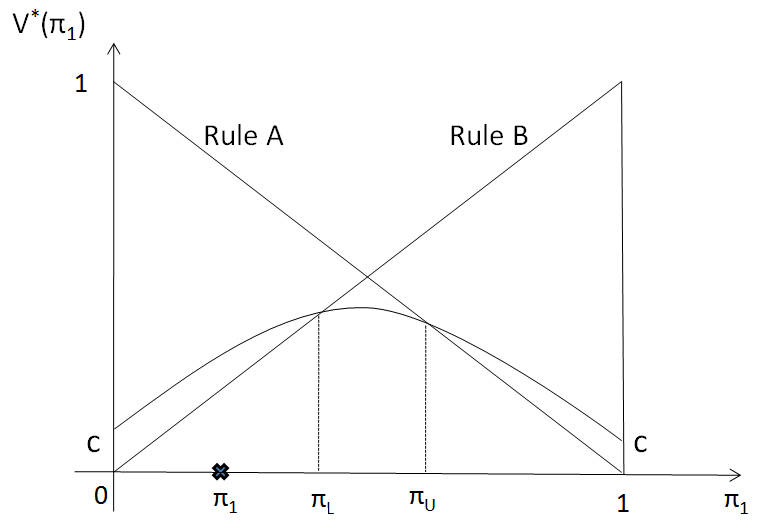
\includegraphics[scale=0.7]{Figures/BayesRisk_2017.png}
	\caption{Bayes Risk for different rules: $ (i)$ Rule A: $ \phi_0=1, \delta_0=1$, $(ii)$ Rule B: $\phi_0=1, \delta_0=0$.}	
	\label{fig:BayesRisk}	
\end{figure}

\noindent From figure \ref{fig:BayesRisk}, it follows that:\\
Case 1: If $\pi_1 \leq \pi_L$, then Bayes rule is: $(\phi_0=1, \delta_0=1)$\\
Case 2: If $\pi_1 \geq \pi_u$, then the Bayes rule is: $(\phi_0=1, \delta_0=1)$\\
Case 3: if $\pi_L \le \pi_1 \le \pi_u$, then $\phi_0=0$\\
\newline
Update pair ($\pi_0,\pi_1$) using observation $Y_1=y_1$ and Bayes formula,\newline\\
$\pi_1$($y_1$) = P[$H_1$ is true/$Y_1$=$y_1$]  (Posterior probability of $H_1$ given $Y_1$=$y_1$) \newline
$\pi_0$($y_1$) = 1- $\pi_1$($y_1$)\newline
Use the same idea to decide $\phi_1$($y_1$) = 0 or 1 based on $\pi_1$($y_1$)

\section{The Optimal Bayes Rule}
(Proof not presented)\newline

The optimal rule is:
\begin{eqnarray}
\label{l10}
\phi_n(y_1,y_2,\cdots,y_n) =  
\begin{cases}
0 \ \ \ \ if \ \pi_1(y_1,y_2,\cdots,y_n)\in[\pi_L,\pi_u] \\
1 \ \ \ \ if \ otherwise
\end{cases}
\end{eqnarray}

\begin{eqnarray}
\label{l10}
\delta_n(y_1,y_2,\cdots,y_n) =  
\begin{cases}
0 \ \ \ \ if \ \pi_1(y_1,y_2,\cdots,y_n)\leq\pi_L \\
1 \ \ \ \ if \ \pi_1(y_1,y_2,\cdots,y_n)\geq\pi_u \\
0 \ or \ 1 \ \ if \ otherwise\ (doesn't \ matter!)
\end{cases}
\end{eqnarray}


\begin{figure}
	\centering
	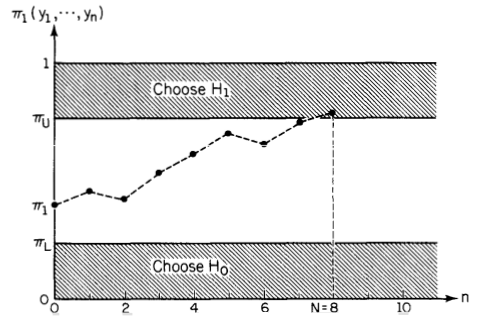
\includegraphics[scale=0.7]{Figures/bayesseqtest.png}\\
	\caption{Depiction of realization of a Bayes sequential test}
\end{figure}
%$\pi_1$$(y_1,y_2,\cdots,y_n)$ = P($H_1$ is true/$Y_1=y_1,Y_2=y_2,\cdots, %Y_n=y_n$)\newline
\begin{eqnarray}
\pi_1(y_1,y_2,\cdots,y_n)&=&P(H_1 \ is \ true/Y_1=y_1,Y_2=y_2,\cdots, Y_n=y_n)\\
&=&\frac{P(Y_1=y_1,Y_2=y_2,\cdots, Y_n=y_n/H_1)P(H_1)}{\sum_{j=0}^{1}P(Y_1=y_1,,\cdots, Y_n=y_n/H_j)P(H_j)}\\
&=&\frac{\pi_1\prod_{k=1}^{n}P_1(y_k)}{\sum_{j=0}^{1}\pi_j\prod_{k=1}^{n}P_j(y_k)}\\
&=&\frac{\pi_1L_n(Y_1=y_1,Y_2=y_2,\cdots, Y_n=y_n)}{\pi_1L_n(Y_1=y_1,Y_2=y_2,\cdots, Y_n=y_n)+\pi_0}
\end{eqnarray}
where 
\begin{eqnarray}
L_n(Y_1=y_1,Y_2=y_2,\cdots, Y_n=y_n)=\prod_{k=1}^{n}\frac{P_1(y_k)}{P_0(y_k)}
\end{eqnarray}

\noindent Unfortunately, $\pi_L$ and $\pi_u$ are not easily computable!\newline
We can rewrite the optimal Bayes rule as:\newline

\begin{eqnarray}
%\label{l10}
\phi_n(y_1,y_2,\cdots,y_n) =  
\begin{cases}
0 \ \ \ \ if \ L_n\in [\underline{\pi},\overline{\pi}] \\
1 \ \ \ \ otherwise\\
\end{cases}
\end{eqnarray}

\begin{eqnarray}
%\label{l10}
\delta_n(y_1,y_2,\cdots,y_n) =  
\begin{cases}
0 \ \ \ \ if \ L_n\leq \underline{\pi} \\
1 \ \ \ \ if \ L_n \geq\overline{\pi} \\
0 \ or \ 1 \ \ if \ otherwise\ (doesn't \ matter!)
\end{cases}
\end{eqnarray}

where\newline
\begin{eqnarray}
\underline{\pi}=\frac{\pi_0\pi_L}{\pi_1(1-\pi_L)}\\
\overline{\pi}=\frac{\pi_0\pi_u}{\pi_1(1-\pi_u)}
\end{eqnarray}

In general, we can consider the class of sequential decision rules, called Sequential Probability Ratio Tests (SPRT(a,b)), a$\leq$ b.\\\newline
\noindent \textbf{\underline{NOTE:-}} \nonumber\\

$L_0$=0 By definition.\newline

SPRT(a,b): Take samples until\newline
\begin{eqnarray}
L_n(y_1,y_2,\cdots,y_n)>b \ \ : Returns \ \ H_1\\ 
L_n(y_1,y_2,\cdots,y_n)<a \ \ : Returns \ \ H_0
\end{eqnarray}
\end{document}